% !TEX root = ../SYSprojektrapport.tex
% SKAL STÅ I TOPPEN AF ALLE FILER FOR AT MASTER-filen KOMPILERES 

\label{Validering}
\section{Validering}

For at sikre at PowerFactory modellen af det dansk elnet, er designet som forventet er der blevet gennemført en validering af modellen. Validering er lavet på baggrund af en spændingsfaldsberegninger og en kortslutningsberegninger. I valideringen forsyner den synkrone generatorenhed hele nettet og belastningsforholdet er designet således der er overenstemmelse mellem produktion og belastning. Vindmølleparken er koblet ud ved \textit{Transmission central 160kV busbar} og alle batterier og solceller er koblet ud ved deres POC. Ydermere er evt. ringforbindelser og redundant forbindelser koblet ud, således at kun \textit{Town3} forsynes direkte fra \textit{Distribution busbar}. Se figur \ref{fig:Simdis} og \ref{fig:SimTrans} for referencer.

\subsection{Validering med spændingsfaldsberegninger}
Spændingsfaldet blev beregnet på 10kV distributionsbusbaren. Dette blev gjort ved at beregne impedansen for alle dele af modellen. Herunder er et beregningseksempel for hvert elnet element i valideringsmodellen.

Synkron generator:
\begin{figure}[H] % (alternativt [H])
	\centering
	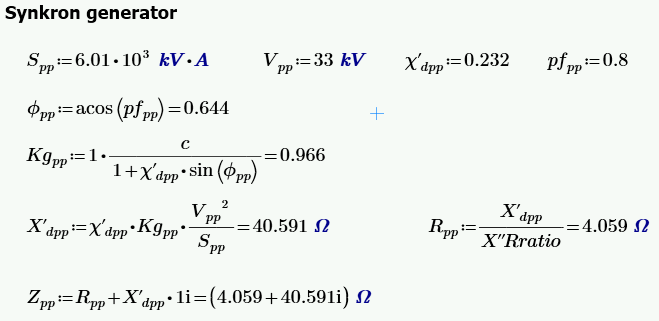
\includegraphics[width=0.85\textwidth]{figurer/Synkron_generator_validering}
	\caption{Synkron generator impedans}
	\label{fig:SGimpedans}
\end{figure}

Transformer:
\begin{figure}[H] % (alternativt [H])
	\centering
	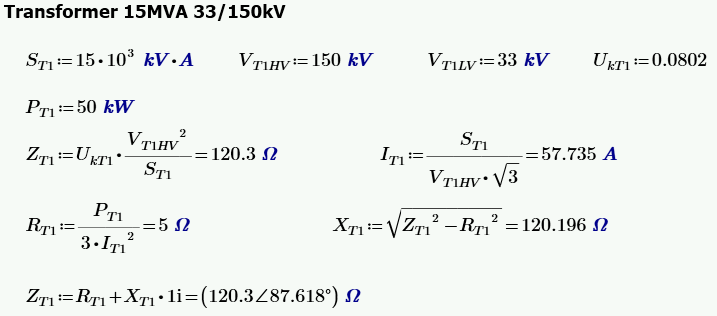
\includegraphics[width=0.9\textwidth]{figurer/Transformer_validering}
	\caption{Transformer impedans}
	\label{fig:Trafoimpedans}
\end{figure}

Kabel:
\begin{figure}[H] % (alternativt [H])
	\centering
	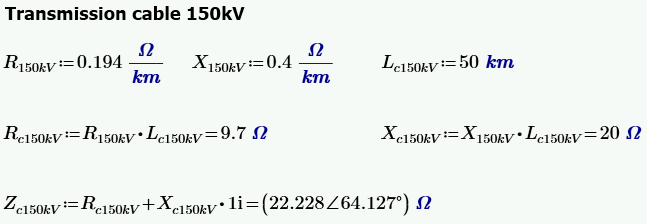
\includegraphics[width=0.8\textwidth]{figurer/Kabel_validering}
	\caption{Kabel impedans}
	\label{fig:Kabelimpedans}
\end{figure}

Byer:
\begin{figure}[H] % (alternativt [H])
	\centering
	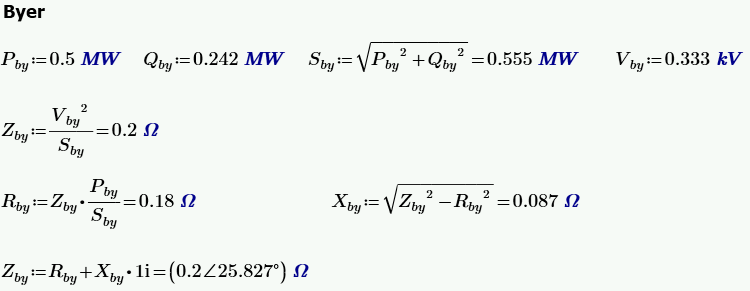
\includegraphics[width=0.9\textwidth]{figurer/By_validering}
	\caption{By impedans ved simuleringsspænding}
	\label{fig:Byimpedans}
\end{figure}

 Når impedansen for alle elementer i valideringssimuleringen er beregnet kan man beregne spændingsfaldet ved en bestemt busbar. \textit{Distribution busbar} blev brugt til validering. $Z_{source}$ dækker her over alle impedanser før 10kV distributionsbusbaren og $Z_{load}$ dækker over alle impedanser efter \textit{Distribution busbar}. $V_{T4HV}$ er 10kV.
 
 \begin{figure}[H] % (alternativt [H])
 	\centering
 	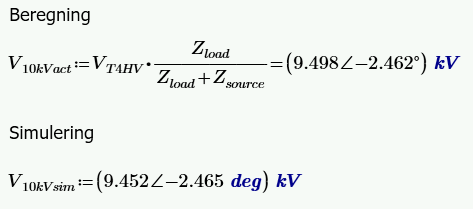
\includegraphics[width=0.6\textwidth]{figurer/Spaendingsfald_validering}
 	\caption{Spændingsfald ved beregning og simulering}
 	\label{fig:Spaendingsfald_validering}
 \end{figure}
 
 Som det ses på figur \ref{fig:Spaendingsfald_validering} er afvigelsen mellem beregning og simulering 46V vinkel 0.003deg, som er en tilladelig afvigelse på et 10kV referencepunkt. Ud fra spændingsfaldsvalidering er modellen dermed accepteret.
 
\subsection{Validering med kortslutningsberegninger}
Kortslutningsberegninger er også beregnet for \textit{Distribution busbar}. Dette gøres ved at finde kortslutningsimpedansen, der er den samme som $Z_{source}$, bortset fra at synkron generatorens kortslutningseffekt er større end dens rated effekt og dermed ses en mindre kildeimpedans for synkron generatoren. Den nye beregning for synkron generator impedansen ses på figur \ref{fig:SGimpedansSC}.

\begin{figure}[H] % (alternativt [H])
	\centering
	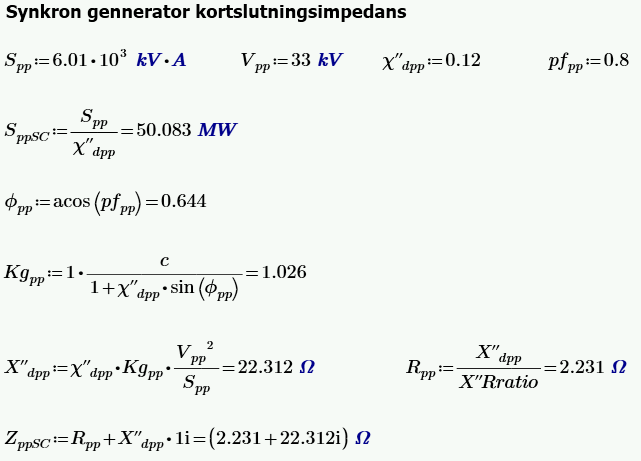
\includegraphics[width=0.75\textwidth]{figurer/Synkron_generator_valideringSC}
	\caption{Synkron generator kortslutningsimpedans}
	\label{fig:SGimpedansSC}
\end{figure}

Derefter kan kortslutningsstrømmen ved en trefaset kortslutning på \textit{Distribution busbar} beregnes, samt findes ved simulering.

\begin{figure}[H] % (alternativt [H])
	\centering
	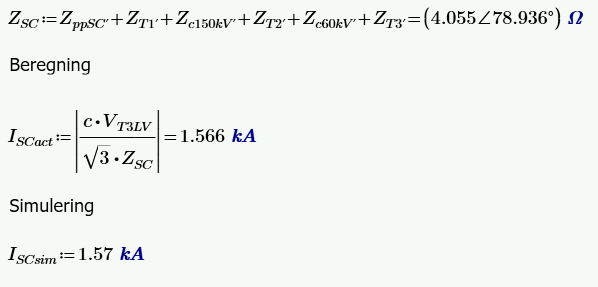
\includegraphics[width=0.75\textwidth]{figurer/Kortslutningsstroem_validering}
	\caption{Kortslutningsstrøm ved beregning og simulering}
	\label{fig:SCvalidering}
\end{figure}

På figur \ref{fig:SCvalidering} ses det at forskellen på beregning og simulering kun er 4A. Derfor accpeteres modellen også gennem validering med kortslutningsberegninger.



\subsection{Resultat af validering}

Udfra de beskrevne resultater i begge dele af valideringen, er der opnåede acceptable afvigelser mellem beregning og simulering. Derfor accepteres modellen til videre simuleringen af de tidligere nævnte projekt cases.